\documentclass[tikz,border=2pt]{standalone}
\usepackage{amsmath,amssymb}
\usepackage{pgfplots}
\pgfplotsset{compat=1.18}

\begin{document}
% Discrete H, continuous Y: H ~ Bern(1/2), Y | H=0 ~ Exp(1), Y | H=1 ~ Exp(2). The posterior
% P(H=1 | Y=y) = 2e^{-2y}/(e^{-y}+2e^{-2y}) falls from 2/3; at y = ln 2 the two densities are equal.
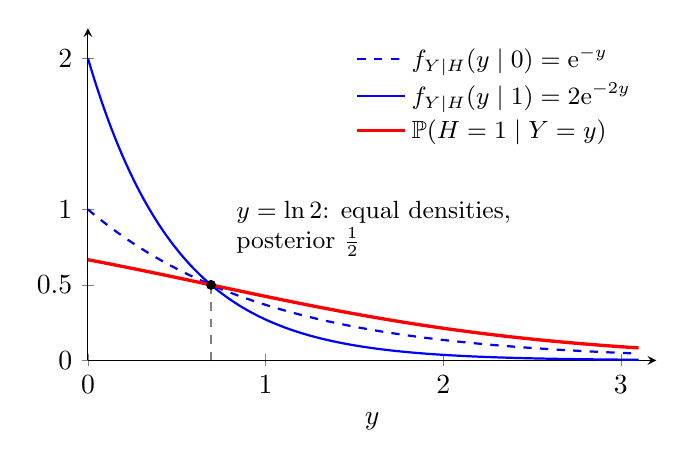
\begin{tikzpicture}
	\begin{axis}[
		axis lines=left, xmin=0, xmax=3.2, ymin=0, ymax=2.2,
		xtick={0,1,2,3}, ytick={0,0.5,1,2},
		xlabel={$y$}, samples=120, smooth,
		width=8.8cm, height=5.8cm, clip=false,
		legend style={draw=none, fill=none, font=\small, at={(0.98,0.98)}, anchor=north east}, legend cell align=left
		]
		\addplot[blue, thick, dashed, domain=0:3.1] {exp(-x)};
		\addlegendentry{$f_{Y\mid H}(y\mid0)=\mathrm{e}^{-y}$}
		\addplot[blue, thick, domain=0:3.1] {2*exp(-2*x)};
		\addlegendentry{$f_{Y\mid H}(y\mid1)=2\mathrm{e}^{-2y}$}
		\addplot[red, very thick, domain=0:3.1] {2/(exp(x)+2)};
		\addlegendentry{$\mathbb{P}(H=1\mid Y=y)$}
		\draw[gray, dashed] (axis cs:0.693,0) -- (axis cs:0.693,0.5);
		\fill[black] (axis cs:0.693,0.5) circle (1.8pt);
		\node[anchor=south west, font=\small, align=left] at (axis cs:0.78,0.62) {$y=\ln2$: equal densities,\\ posterior $\tfrac12$};
	\end{axis}
	
\end{tikzpicture}
\end{document}
